\documentclass{beamer}
\usepackage[T1]{fontenc}
\usepackage[utf8]{inputenc}
\usepackage{lmodern}
\usepackage[ngerman]{babel}

\usepackage{graphics}

\usepackage{amsmath}
\usepackage{booktabs}
\usepackage{listings}

\usepackage{dot2texi}
\usepackage{tikz}
\usetikzlibrary{arrows,shapes}
 \usetikzlibrary{matrix}
\usetikzlibrary{automata}

\usepackage{wrapfig}

\usetheme{Singapore}
\usecolortheme{dove}
\graphicspath{{images/}{../comics/}}

\newcommand{\xn}{\visible<2->{$\times$}}
\newcommand{\xj}{\visible<2->{$\checkmark$}}
\newcommand{\rd}[1]{\textcolor{red}{#1}}
\newcommand{\gn}[1]{\textcolor{green}{#1}}
\newcommand{\bl}[1]{\textcolor{blue}{#1}}

\newcommand{\hiddencell}[2]{\action<#1->{#2}}

\newcommand{\link}[2][blue]{\underline{\textcolor{#1}{#2}}} 	% \link{www.example.org} zeigt www.example.org in blau und unterstrichen
\renewcommand{\emph}[1]{\textit{\textcolor{blue}{#1}}}			% \emph{Test} zeigt Text in blau und kursiv
\newcommand{\warn}[1]{\textcolor{red}{#1}}			% \warn{Warning} zeigt Warning in rot und kursiv

\AtBeginSection[]
{
  \begin{frame}[plain]
    \frametitle{}
    {\footnotesize
      \tableofcontents[currentsection]
    }
  \end{frame}
}

\title{Grundbegriffe der Informatik}
\author{Patrick Niklaus}

\begin{document}
\begin{frame}
  \frametitle{Grundbegriffe der Informatik}
  \framesubtitle{7. Tutorium}
  \begin{description}
    \item \textbf{Name:} Patrick Niklaus
    \item \textbf{E-Mail:} patrick.niklaus@student.kit.edu
    \item \textbf{Nr:} 43
  \end{description}
\end{frame}

\section{Übungsblatt}
\begin{frame}
  \frametitle{Anmerkungen zum letzten Übungsblatt}
  \begin{enumerate}
    \item Beweise sind systematische Begründungen. "`geht nicht"' ist keine Begründung.
    \item Ein geschlossener Pfad/Weg hat immer den gleichen Anfangs- und Endknoten.
  \end{enumerate}
\end{frame}

\section[Effizienz]{Algorithmen-Effizienz}
\subsection{Motivation}
\begin{frame}
  \frametitle{Effizienzberechnung}
  \begin{block}{Problem}
    \begin{itemize}
      \item Ist ein Algorithmus besser als ein anderer?
      \item Gilt das auch auf einer anderen Rechenmaschine?
      \item Gilt es auch, wenn die Datenmenge weiter wächst?
    \end{itemize}
  \end{block}
  \pause
  \begin{block}{Lösungsansatz}
    Wir abstrahieren die Effizienz von Algorithmen:
    \begin{itemize}
      \item unabhängig von der Rechenmaschine
      \item in Abhängigkeit der Eingabelänge (meist $n$)
      \item mathematisch fundiert und beweisbar
    \end{itemize}
  \end{block}
\end{frame}
\begin{frame}
  \frametitle{Laufzeitfunktion}
  \begin{itemize}
    \item Wie kann sagen: "`Ein Algorithmus braucht mehr Zeit zum berechnen als ein anderer?"'
    \item Wir nehmen die Anzahl der \emph{Rechenoperationen} als Maß für "`Zeit"'.
  \end{itemize}
  \pause
  \begin{definition}
    Sei $t: \mathbb{N} \longrightarrow \mathbb{R}^+$ eine Funktion, die von der Größe der Eingabe $n$ auf die Anzahl der Operationen eines Algorithmus abbildet.
    $t$ heißt dann \emph{Laufzeitfunktion}.
  \end{definition}
\end{frame}

\subsection{Das O-Kalkül}
\begin{frame}
  \frametitle{$O$-Kalkül}
    \begin{block}{Definition}
          $O(g(n)): =\{\ f(n)\ |\ \exists c \in \mathbb{R}^+ \exists n_{0} \in \mathbb{N}\ \forall n \ge n_{0}:$\\
          \hspace{9em} $0 \le f(n) \le c\cdot g(n)\ \}$
    \end{block}

  \begin{alertblock}{Umgangssprachlich}
    $O(g(n))$ enthält alle nicht-negativen Funktionen, die höchstens so schnell wie $g(n)$ wachsen.
    Wir vernachlässigen:
    \begin{itemize}
      \item was am Anfang passiert ($\exists n_0\in\mathbb{N}$ \ldots $\forall n\ge n_0$).
      \item einfache Faktoren ($\exists c\in\mathbb{R}^+$ \ldots $c\cdot g(n)$).
    \end{itemize}
  \end{alertblock}
\end{frame}

\begin{frame}
  \frametitle{Rechnen mit Mengen}
  \begin{definition}
    Seien $M_1, M_2$ zwei Mengen. Wir definieren:
    \begin{description}
      \item $M_1 + M_2 := \{m_1 + m_2 : \forall m_1 \in M_1, m_2 \in M_2\}$
      \item $M_1 \cdot M_2 := \{m_1 \cdot  m_2 : \forall m_1 \in M_1, m_2 \in M_2\}$
    \end{description}
    Für $M_1 = \{x\}$ kann man dann auch schreiben:
    \begin{description}
      \item $x + M_2 := \{x\} + M_2$
      \item $x \cdot M_2 := \{x\} \cdot M_2$
    \end{description}
  \end{definition}
\end{frame}

\begin{frame}
  \frametitle{Rechnen mit dem $O$-Kalkül}
  \begin{block}{Wichtige Regeln}
    \begin{enumerate}
      \item $O(1) + O(23) + O(4) = O(1)$
      \item $O( f(n) ) + O( f(n) ) = O( f(n) )$
      \item $O( a\cdot f(n) ) = O(f(n)) \ \forall a\in\mathbb{R}$
      \item $O( a\cdot n^2+b\cdot n+c ) = O( n^2 ) \ \forall a,b,c\in\mathbb{R}$
    \end{enumerate}
  \end{block}
  \begin{alertblock}{Faustregel}
    "`Der Stärkere gewinnt!"'
  \end{alertblock}
\end{frame}

\subsection{Aufwandsklassen}

\begin{frame}
  \frametitle{Aufwandsklassen}
  \begin{description}
    \item[$f(n) \in O(g(n))$]  \hfill \\
      "`f wächst asymptotisch höchstens so viel wie g"'
    \item[$f(n) \in \Omega(g(n))$] \hfill \\
      "`f wächst asymptotisch ungefähr so viel wie g"'
    \item[$f(n) \in \Theta(g(n))$] \hfill \\
      "`f wächst asymptotisch mindestens so viel wie g"'
  \end{description}
\end{frame}

\begin{frame}
			\frametitle{Aufwandsklassen}
		\only<1>{
				Obere asymptotische Schranke\\
				$O(g(n)) := \{f(n) \,|$\\$ \exists c \in \mathbb{R}^+, n_0 \in \mathbb{N} \,\forall n > n_0 : 0 \leq f (n) \leq c \cdot g(n)\}$\\
\vspace{3ex}
				Untere asymptotische Schranke\\
				$\Omega(g(n)) := \{f (n) \,|$\\$ \exists c \in \mathbb{R}^+, n_0 \in \mathbb{N} \,\forall n > n_0 : 0 \leq c \cdot g(n) \leq f (n)\}$\\
\vspace{3ex}
				Asymptotisch scharfe Schranke\\
				$\Theta(g(n)) := \{f (n) \,|$\\$ \exists c_1, c_2 \in \mathbb{R}^+, n_0 \in \mathbb{N} \,\forall n > n_0 :
					0 \leq c_1 \cdot g(n) \leq f (n) \leq c_2 \cdot g(n)\}$\\
		}
		\begin{alertblock}{Beachte:}
		  Alle Kalküle geben eine \emph{Menge} von Funktionen an.
    \end{alertblock}
\end{frame}


\begin{frame}
  \frametitle{O-Kalkül}
  \begin{figure}[hgtb]
    \begin{center}
    \includegraphics[width=200pt]{images/o.pdf}
    \end{center}
  \end{figure}
\end{frame}
\begin{frame}
  \frametitle{$\Omega$-Kalkül}
  \begin{figure}[hgtb]
    \begin{center}
    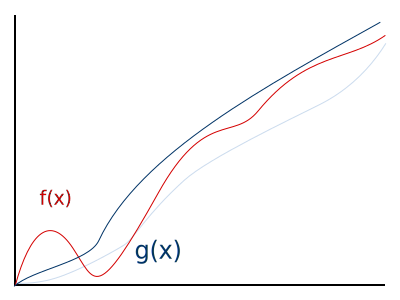
\includegraphics[width=200pt]{images/omega.pdf}
    \end{center}
  \end{figure}
\end{frame}
\begin{frame}
  \frametitle{$\Theta$-Kalkül}
  \begin{figure}[hgtb]
    \begin{center}
    \includegraphics[width=200pt]{images/theta.pdf}
    \end{center}
  \end{figure}
\end{frame}

\subsection{Rechenregeln}
\begin{frame}
  \frametitle{Rechenregeln}
	\begin{block}{Reflexivität}
    \begin{itemize}
      \item $f(n) \in O(f(n))$
      \item $g(n) \in \Omega(g(n))$
      \item $h(n) \in \Theta(h(n))$
    \end{itemize}
	\end{block}
	\begin{block}{Symmetrie}
	 Hier gilt nur:  $f(n) \in \Theta(g(n)) \Leftrightarrow g(n) \in \Theta(f(n))$
	\end{block}
	\begin{block}{Der Stärkere gewinnt.}
    \begin{itemize}
      \item $O(n^2 + n + log(n)) = O(n^2)$
          \item $\Omega(n^2 + n + log(n)) = \Omega(n^2) \subset \Omega(log(n))$
    \end{itemize}
  \end{block}
\end{frame}

\subsection{Beispiele}
\begin{frame}[plain]
		\frametitle{Ausführliches Beispiel}
		Behauptung: $n^2 + n \in O(n^2)$\\
    Beweis: $n^2 + n \in O(n^2)$\\
			\hspace{2em} $\Leftrightarrow \exists c \in \mathbb{R}^+, n_0 \in \mathbb{N} \,\forall n > n_0 : 0 \leq n^2+n \leq c \cdot n^2 $
		\begin{description}
			\item[Vermutung:] $ c = 2, n_0 = 2$
			\item[I.A.:] $n=2$ : \hfill \\ $ 0 \leq n^2+n = 2^2+2 = 6 \leq 8 = 2 \cdot 2^2 = 2n^2$
			\item[I.V.:] $0 \leq n^2+n \leq 2n^2$
			\item[I.S.:] $n \rightarrow n+1$ :\\ $ 0 \leq (n+1)^2 + (n+1) = n^2 + 3n + 2 \leq 2n^2 + 4n + 2 = 2(n+1)^2 \hfill \blacksquare$
		\end{description}
\end{frame}

\begin{frame}
  \frametitle{Logarithmen}
  \begin{alertblock}{Alle Logarithmen haben asymptotisch das gleiche Wachstum}
    Also: $\log_b(n) \in\Theta(\log_a(n))$ für alle $a, b \in \mathbb{R^+}$.\\
    Man kann also einfach $\Theta(\log n)$ ohne Basis schreiben.
  \end{alertblock}
  $\Rightarrow$ Beweis?
\end{frame}

\subsection{Aufgaben}
\begin{frame}
	\frametitle{Aufgaben}
  Zeigt oder wiederlegt:
  \begin{enumerate}
    \item $f(n) \in O(g(n))$ und $f(n) \in \Omega(g(n))$ folgt: $f(n) \in \Theta(g(n))$
    \item $f(n) \in \Omega(g(n))$ und $g(n) \in O(h(n))$ folgt: $f(n) \in O(h(n))$
  \end{enumerate}
\end{frame}

\begin{frame}
	\frametitle{Aufgaben}
	Welche Funktionen gehören in welche Klassen?
	\begin{Large}
    \begin{center}
      \begin{tabular}{l|c|c|c|c}
                    & $O(n^2)$ & $\Omega(n^2)$ & $O(\log{n})$ & $\Theta(n)$\\ \hline
        $n^2 + n$	  & \xj & \xj & \xn & \xn \\ \hline
        $n \cdot \log(n)$ & \xj & \xn & \xn & \xn \\ \hline
        $2 \cdot n + 1$	  & \xj & \xn & \xn & \xj \\ \hline
        $n^3$		  & \xn & \xj & \xn & \xn \\ \hline
        $5$		  & \xj & \xn & \xj & \xn
      \end{tabular}
    \end{center}
	\end{Large}
\end{frame}

\begin{frame}
	\frametitle{Aufgaben}
  Zeigt oder wiederlegt:
  \begin{enumerate}
    \item $n^2 \in O(n \cdot log(n))$
    \item $4^n \in \Theta(2^n)$
    \item $n \in \Omega(log(n))$
    \item $n^3 \in O(sqrt(2^n))$
  \end{enumerate}
\end{frame}


\section{Abschluss}
\subsection{Zusammenfassung}
\begin{frame}
  \frametitle{Was ihr jetzt wissen sollte.}
  \begin{enumerate}
    \item Wie ist $O(f(n))$, $\Theta(f(n))$ und $\Omega(f(n))$ definiert?
    \item Was sagen sie jeweils mathematisch aus?
    \item Was sagen sie für die Laufzeit eines Algorithmus aus?
  \end{enumerate}
\end{frame}

\subsection{xkcd}
\begin{frame}[plain]
  \begin{figure}
    \begin{center}
      \includegraphics[width=200pt]{tabletop_roleplaying}
    \end{center}
    {\tiny I may have also tossed one of a pair of teleportation rings into the ocean, with interesting results.}
  \end{figure}
\end{frame}

\end{document}
